\documentclass[a4paper,12pt]{report}
\addtolength{\oddsidemargin}{-1.cm}
\addtolength{\textwidth}{2cm}
\addtolength{\topmargin}{-2cm}
\addtolength{\textheight}{3.5cm}
\newcommand{\HRule}{\rule{\linewidth}{0.5mm}}
\makeindex

\usepackage{longtable}
\usepackage[pdftex]{graphicx}
\usepackage{makeidx}
\usepackage{hyperref}
\hypersetup{
    colorlinks=true,
    linkcolor=blue,
    filecolor=magenta,      
    urlcolor=cyan,
}


% define the title
\author{Men-at-Work}
\title{ OnlyRugby Functional Requirements}
\begin{document}
\setlength{\parskip}{6pt}

% generates the title
\begin{titlepage}

\begin{center}
% Upper part of the page       

\includegraphics[width=1\textwidth]{./up-logo.jpg}\\[0.4cm]    
\textsc{\LARGE Department of Computer Science}\\[1.5cm]
\textsc{\Large COS 301 - Software Engineering}\\[0.5cm]
% Title
\HRule \\[0.4cm]
{ \huge \bfseries OnlyRugby Functional Requirements}\\[0.4cm]
\HRule \\[0.4cm]
% Author and supervisor
\begin{minipage}{0.4\textwidth}
\begin{flushleft} \large
\emph{Author:}\\
Herman {Keuris}
\end{flushleft}
\end{minipage}
\begin{minipage}{0.4\textwidth}
\begin{flushright} \large
\emph{Student number:} \\
u13037618
\end{flushright}
\end{minipage}
\begin{minipage}{0.4\textwidth}
\begin{flushleft} \large
Johan {van Rooyen}
\end{flushleft}
\end{minipage}
\begin{minipage}{0.4\textwidth}
\begin{flushright} \large
\emph{} \\
u11205131
\end{flushright}
\end{minipage}
\begin{minipage}{0.4\textwidth}
\begin{flushleft} \large
Estian {Rosslee}
\end{flushleft}
\end{minipage}
\begin{minipage}{0.4\textwidth}
\begin{flushright} \large
\emph{} \\
u12223426
\end{flushright}
\end{minipage}
\begin{minipage}{0.4\textwidth}
\begin{flushleft} \large
Ivan {Henning}
\end{flushleft}
\end{minipage}
\begin{minipage}{0.4\textwidth}
\begin{flushright} \large
\emph{} \\
u13008219
\end{flushright}
\end{minipage}
\begin{minipage}{0.4\textwidth}
\begin{flushleft} \large
Muller {Potgieter}
\end{flushleft}
\end{minipage}
\begin{minipage}{0.4\textwidth}
\begin{flushright} \large
\emph{} \\
u12003672
\end{flushright}
\end{minipage}
\vfill
% Bottom of the page
{\large \today}
\end{center}
\end{titlepage}
\footnotesize
%\input{declaration_of_originality.tex}
\normalsize

\renewcommand{\thesection}{\arabic{section}}
\newpage
\begin{center}
\textsc{\LARGE Software Requirements Specification and Technology Neutral Process Design}\\[1.5cm]
\textsc{\Large OnlyRugby Mobile App/Main Project}\\[0.5cm]
Version: Version 0.2 Alpha 
For further references see \href{ https://github.com/hermankeuris/OnlyRugbyApp.git}{gitHub}.
\today
\end{center}
\tableofcontents{}
\newpage
\section{Functional requirements}
\subsection{Introduction}
The OnlyRugby App will be used to log various types of match time data and then store that information on the OnlyRugby database (which can also be accessed by the OnlyRugby website). The purpose of this document is to identify and explain all possible use cases associated with the app and to show how the functional aspects of the app interact with each other.
% \newpage
\subsection{Use case prioritiation}
\textbf{Critical} 
\begin{itemize}
  \item Log in/log out
  \item Load info (from database)
  \item Game time
  \item Scoring
\end{itemize}
\textbf{Important} 
\begin{itemize}
  \item Substitutions
  \item Discipline
\end{itemize}
\textbf{Nice-To-Have} 
\begin{itemize}
  \item Line-outs
  \item Scrums
  \item Tackles
  \item Possession 
  \item Turn-overs
  \item Clean breaks
  \item Offloads
  \item Rucks
  \item Mauls
\end{itemize}
\newpage
\subsection{Use case/Service contracts}
\begin{center}
  \begin{longtable}{| p{3cm} | p{4cm} | p{4cm} | p{4cm} |}
    \hline
    Use Case & Pre Condition & Post Condition & Description \\ 
    \hline \hline
    Log in/log out & The app has to be connected to the internet in order to verify the information. Only an administrator of a rugby page or user given rights can log in to use the record details part of the app. Once the user is logged in he/she can then use the logout functionality to log out & The user is logged in now and information on upcoming games from the page that the user is a part of should be displayed. The user can then choose the game to record details for. & This use case provides a method for logging in to record match data and log out once done.\\ 
    \hline
    Load info & The app has to be connected to the internet in order to load the info from or to the server (and by extension, the database). Specific info can only be loaded when a person is logged in (like profile information). Statistical information being uploaded needs to know and verify where it is being sent to (i.e. to a player's profile or a team's statistics page). & The information should be loaded into the app from the server and statistical match information should be uploaded and stored in the database via the server, in the correct locations where it is meant to go. This is done by verifying the destination and the data being received each time. & This use case provides a method of uploading and downloading data from the database via the server, to and from the app. \\ 
    \hline
    Game time & The user must be logged in, the app must be aware that a match is scheduled for play and the game state should be "Not started". & The start and end time of each half of the match along with game pause intervals and reasons should be persisted to the database. The game state should be set to "Finished".  & This use case provides an interface for capturing the game time of a rugby match. \\ 
    \hline
    Scoring & The app must be aware that a match is currently being played (i.e. scoring can only occur during game time), the app must be aware of which teams are playing and also be aware of which players are currently on the field (i.e. it must know if any player substitutions have taken place). & All scores must be verified by the user and then uploaded to the database where it can be added to team-, player- and league statistics (including points scored, at what time during the match the points were scored, if it was a try, drop kick, etc). & This use case provides a system whereby event-, team- and player statistics can be gathered during a match so that it can be viewed, analysed and compared with at a later stage.\\ \hline
    Substitutions & The app must be aware that a match is currently being played (although substitutions can still be allowed at half-time). The app must have a list of players currently on the field as well as players in reserve. & After a substitution is made the on-field team and the list of reserve players must be updated accordingly, the time of the substitution will be logged and any special reasons for the substitution (such as injury) will be noted. & This use case provides a way of logging changes in the on-field team (which is important to know for some other functions like Scoring). This use case also provides additional statistical information about the match such as which players were forced off the field due to injury.\\ \hline
	Discipline &  The app must be aware of which teams are playing and also be aware of which players are currently on the field. & After a player has been
given a card, the user must specify the player, the reason for the card and the colour of the card(white/yellow/red). The incident will be added to the relevant
player's profile. & This use case provides a way of quickly logging both the player's infraction and the card reveived.\\ \hline
    Lineouts & The app must be aware that a match is currently in play (i.e. lineouts can only occur during game time) and the app must be aware of which teams are playing. & This function gathers information on when a lineout occurred during game time, which team was responsible for throwing in the ball, the identity of the player throwing in the ball, whether or not the lineout was successful, if successful which team won the lineout, and a reason if the lineout failed. & This use case provides a way of quickly logging information about lineouts.\\ \hline
    Scrums & (Pre conditions) & (Post conditions) & (Description)\\ \hline
    Tackles & The app must be aware that a match is currently being played and have a list of all players (both sides) currently on the field to be able to log tackles made between teams. & The tackler's identity should be verified and the statistics added to the relevant player's profile in the database. & This case provides a way to be able to log how well some players can defend by seeing how many successful tackles they have made throughout their career.\\ \hline
    Possession & The app must be aware that a match is currently being played and know which two teams are currently on the field, in order to log the possession of each team, during the match. & The percentage of each team during the match must be recorded, then logged on the respective teams' profiles & This use case provides a wat of logging a team's posession, during a match.\\ \hline
    Turn-overs & The app must be aware that a match is currently being played and which teams are currently playing (individual players as well). & The name of the player who performed the turn-over must be logged. &  This use case provides a way of quickly logging information about turn-overs.\\ \hline
    Clean breaks & (Pre conditions) & (Post conditions) & (Description)\\ \hline
    Offloads & The app must be aware that a match is currently in play (i.e. offloads can only occur during game time) and the app must be aware of which teams are playing. & The team and identity (name or player number) of the player that made a successful offload should be persisted to the database. & This use case provides a way of quickly logging information about offloads.\\ \hline
    Rucks & The app must be aware that a match is currently being played (i.e. rucks can only occur during game time) and the app must be aware of which teams are playing. & This function gathers information on when a ruck occurred during game time, which team was defending in the ruck and which team "won" the ruck (i.e. if possession of the ball changed then the Possession function will also be notified). & This use case provides a way of quickly logging information about rucks.\\ \hline
    Mauls & The app must be aware that a match is currently being played which teams are currently playing (individual players are not a necessity). & It should be logged which team won the maul and if the ball was turned over (the other team won the ball) or not. & This use case provides a way to represent how many mauls were present in the match, by logging each time a player tried to defend the ball on the ground.\\ \hline

    \hline
  \end{longtable}
\end{center}
\newpage
\subsection{Required functionality}
\begin{itemize}
	% We need to add the correct pictures here. We must also give a description of the elements.
	\item \textbf{Log in/log out}
		\begin{flushleft}
		 The login/logout will be used to let people log in that is an administrator/privileged  user of a rugby page on the onlyRugby site. This will verify if the user has the right credentials to be scoring for a team. Also check the rugby page to see if there are any upcoming games the team will be playing to record the details of the match. 	
		\end{flushleft}
		\begin{center}
  	 	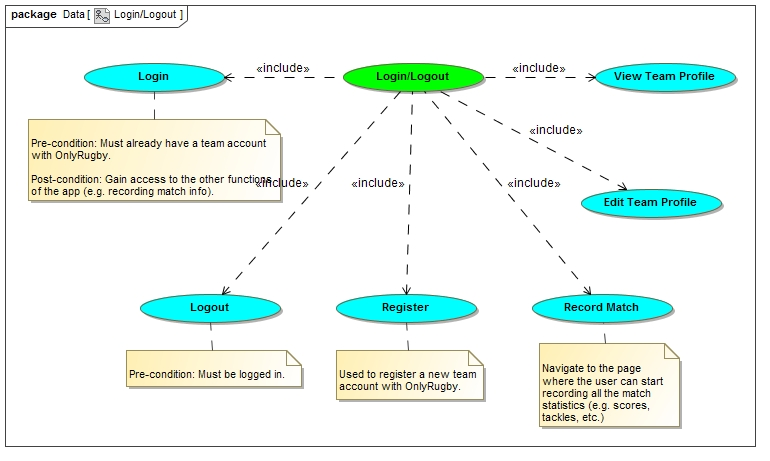
\includegraphics[width=1\textwidth] {./Diagrams/Login_Logout.jpg}\\[0.4cm]    
		\end{center}
\newpage
\item \textbf{Load info}
		\begin{flushleft}
			The Load Info module will be used to transfer information to and from the database, using the server. All destinations are to be verified before attempting to access them and incoming connections to the server need to be verified that they are from a trusted source.
		\end{flushleft}
		\begin{center}
  	 	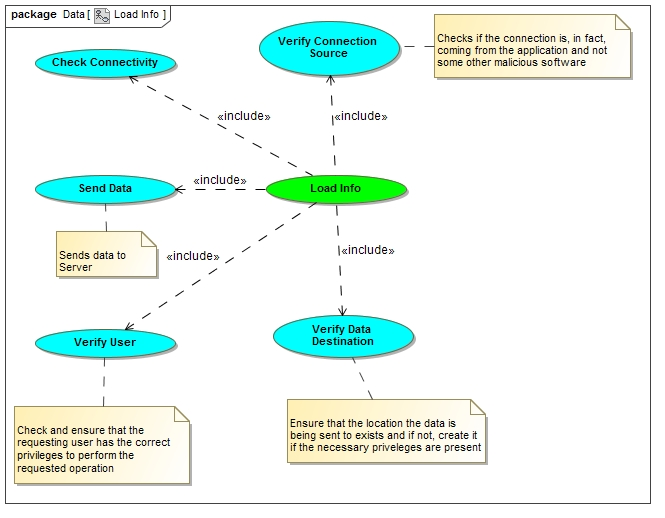
\includegraphics[width=1\textwidth] {./Diagrams/LoadInfo.jpg}\\[0.4cm]    
		\end{center}
\newpage\item  \textbf{Game time}
		\begin{flushleft}
		 This use case will be used to log the start and end time of each half of a match, as well as any intervals during which time was lost (the game was paused) and a reason for this time loss (injury, substitution, referee consultation, replacement of damaged player clothing).	
		\end{flushleft}
		\begin{center}
  	 	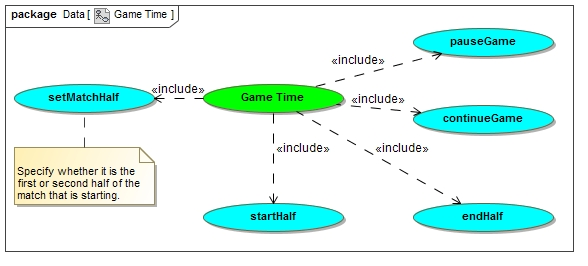
\includegraphics[width=1\textwidth] {./Diagrams/Game Time.jpg}\\[0.4cm]    
		\end{center}
\newpage
\item \textbf{Scoring}
		\begin{flushleft}
		 This use case deals with logging, verifying and storing all the information related to scoring points during a match. When a player scores during a match the app user must use this use case to specify which team scored, the individual player who scored, if the player scored with a try, drop kick, penalty kick or conversion  kick and (in the case of the try) if any other players should be credited with a try assist. This use case will also automatically log when the points were scored. All this information is then verified by the app user before it is stored in the database. Once stored this information can then be used to give team- and player statistics.	
		\end{flushleft}
		\begin{center}
  	 	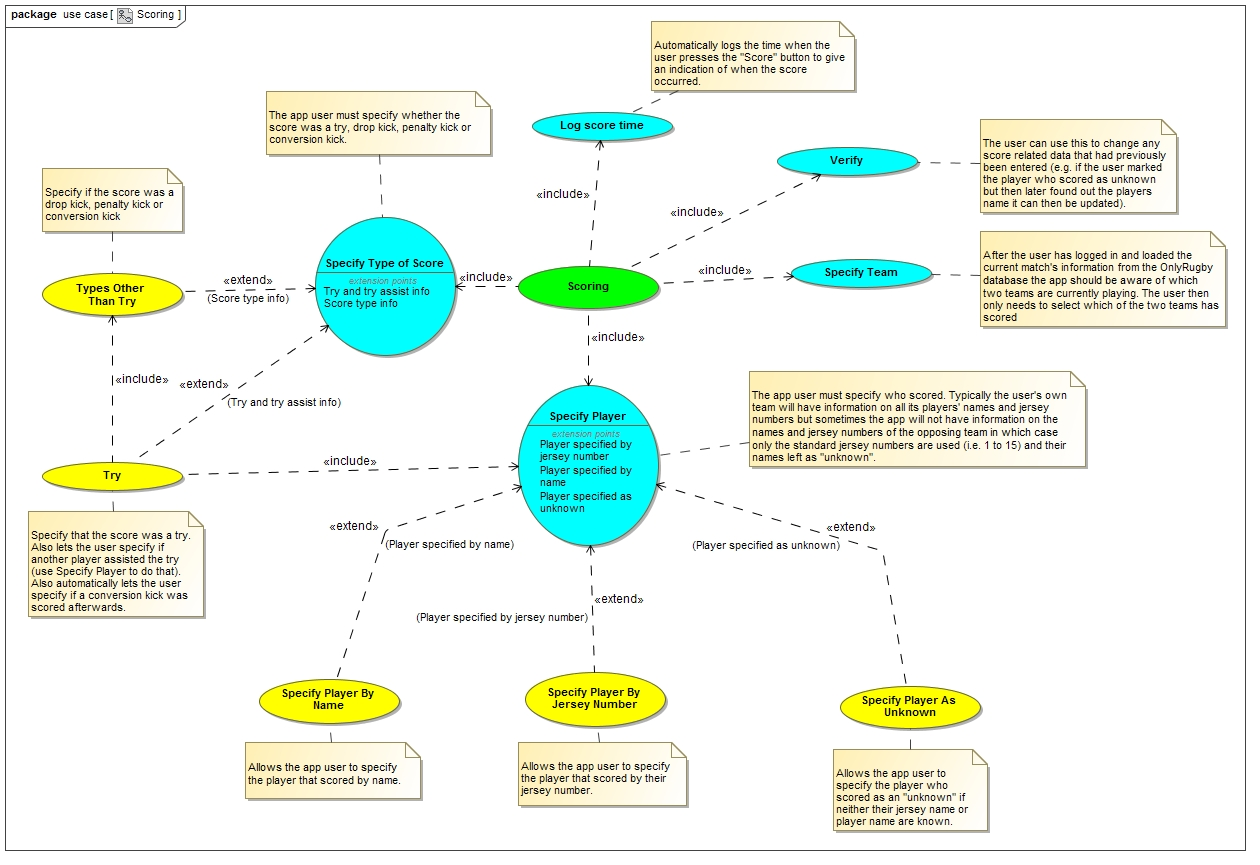
\includegraphics[width=1\textwidth] {./HermanDiagrams/Scoring.jpg}\\[0.4cm]    
		\end{center}
\newpage
	\item \textbf{Substitutions}
		\begin{flushleft}
		 This use case deals with logging and updating any changes made to either teams on-field teams. When a team makes a substitution the user of the OnlyRugby app will use this use case to specify which team made the substitution, which players were swapped and if there was any special reason for the substitution. This use case will also automatically log when a player has been swapped. All this information is then verified by the app user before it is stored in the database. Once stored this information can then be used to give team- and player statistics.
		\end{flushleft}
		\begin{center}
		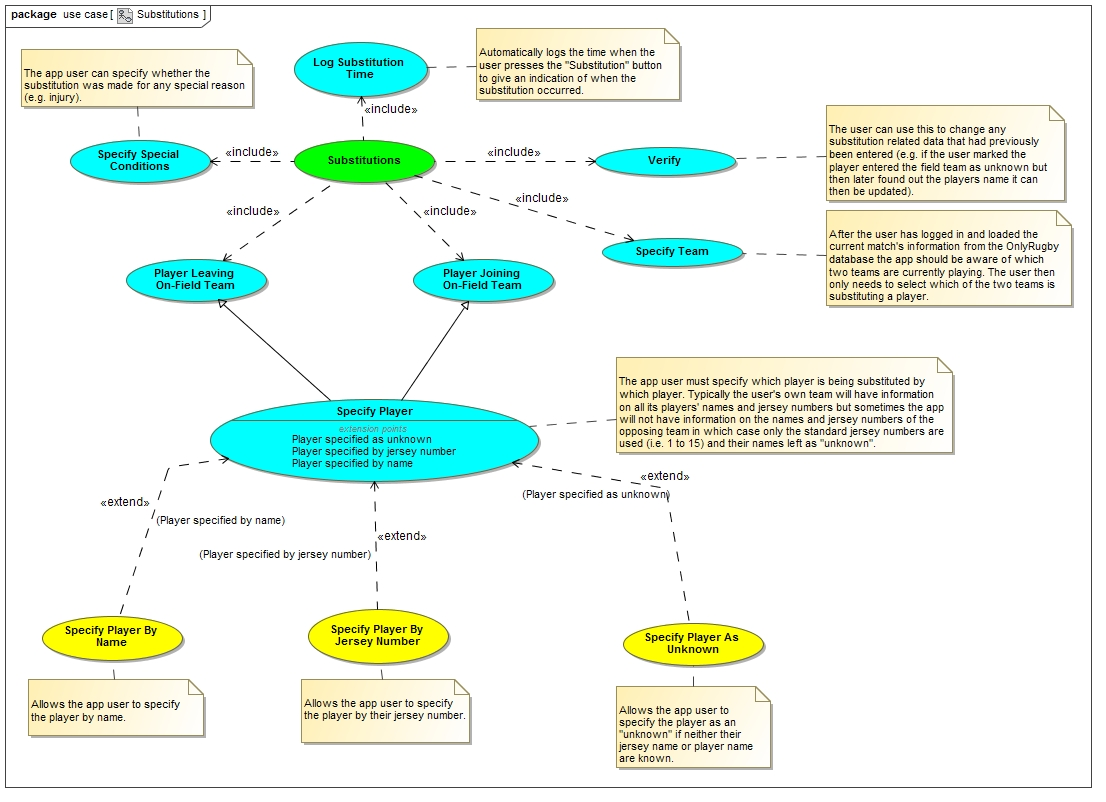
\includegraphics[width=1\textwidth]{./HermanDiagrams/Substitutions.jpg}\\[0.4cm]
		\end{center}
\newpage
	\item \textbf{Discipline}
		\begin{flushleft}
		This use case will be used to log any infractions and subsequent punishment for players. If a player is given a card, the reason for the card, as well as the colour of said card. This data will then be logged to the player's profile.
		\end{flushleft}
		\begin{center}
		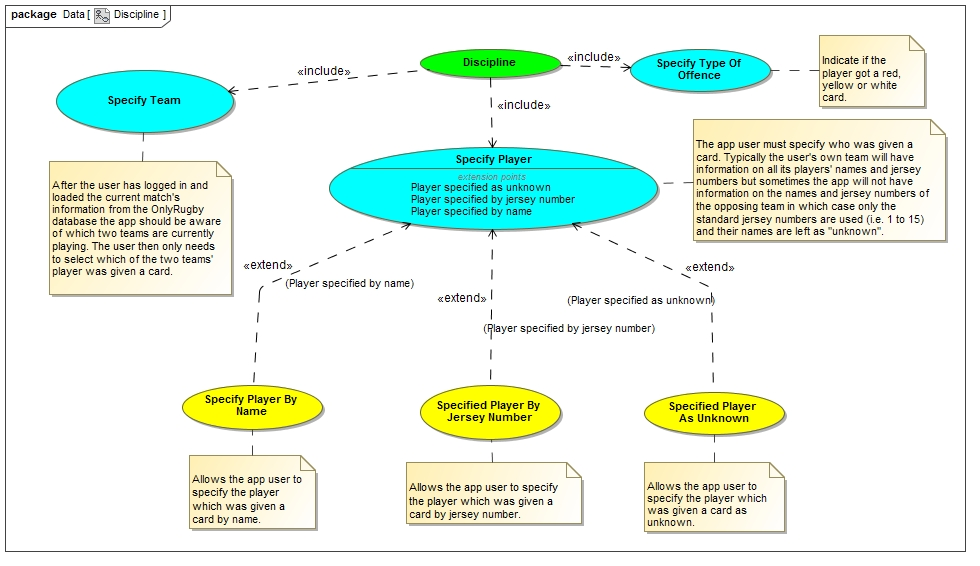
\includegraphics[width=1\textwidth]{./Diagrams/Discipline.jpg}\\[0.4cm]
		\end{center}
\newpage
	\item \textbf{Lineouts}
		\begin{flushleft}
		This use case will be used to log information on when a lineout occurred, which team was responsible for throwing in the ball, the identity (name or player number) of the player that threw in the ball, whether or not the lineout was successful, if successful which team won the lineout, and if unsuccessful a reason why the lineout failed.
		\end{flushleft}
		\begin{center}
		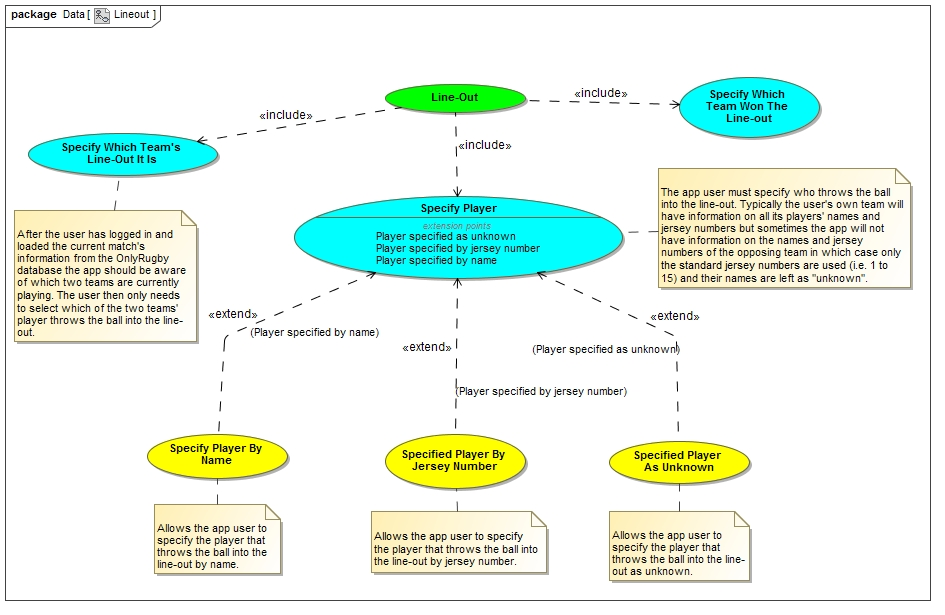
\includegraphics[width=1\textwidth]{./Diagrams/Lineout.jpg}\\[0.4cm]
		\end{center}
\newpage
	\item \textbf{Scrums}
		\begin{flushleft}
		This use case will be used to log information on when a scrum occurred, which team the scrum belonged to and which team won the scrum. The app can check if there are any current reserves on for any forwards or scrum half, and with this info record who was in the scrum.
		\end{flushleft}
		\begin{center}
		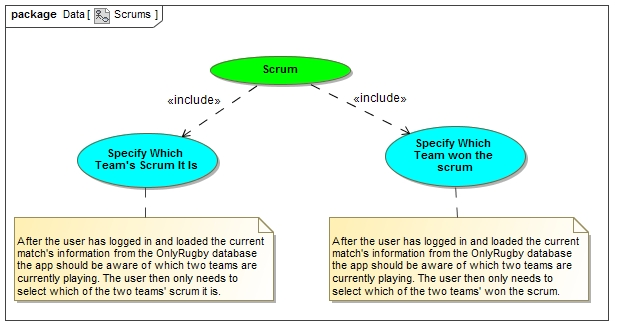
\includegraphics[width=1\textwidth]{./Diagrams/Scrums.jpg}\\[0.4cm]
		\end{center}
	\item \textbf{Tackles}
		\begin{flushleft}
			This use case will be used to log the amount of tackles made, by which team member of which team and when it was made. Knowing who was tackled is not required, since it will not be recorded in their statistics.
		\end{flushleft}
		\begin{center}
		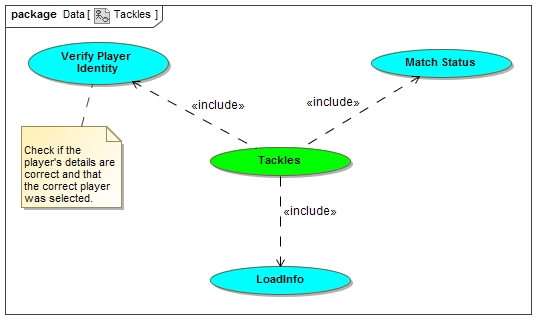
\includegraphics[width=0.9\textwidth]{./Diagrams/Tackles.jpg}\\[0.4cm]
		\end{center}
	\item \textbf{Possession}
		\begin{flushleft}
		This use case will be used to log the percentage of each team's possession for a match. The application will ensure that the total percentages cannot exeed 100 percent.
		\end{flushleft}
		\begin{center}
		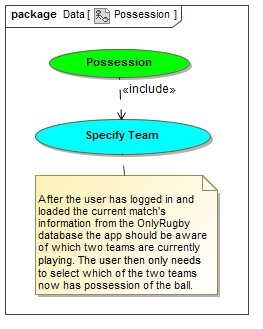
\includegraphics[width=0.4\textwidth]{./Diagrams/Possession.jpg}\\[0.4cm]
		\end{center}
	\item \textbf{Turn-overs}
		\begin{flushleft}
		This use case will be used to log the occurrence of a turn-over, which team got the ball, which team lost the ball and the players who were involved in the turn-over.
		\end{flushleft}
		\begin{center}
		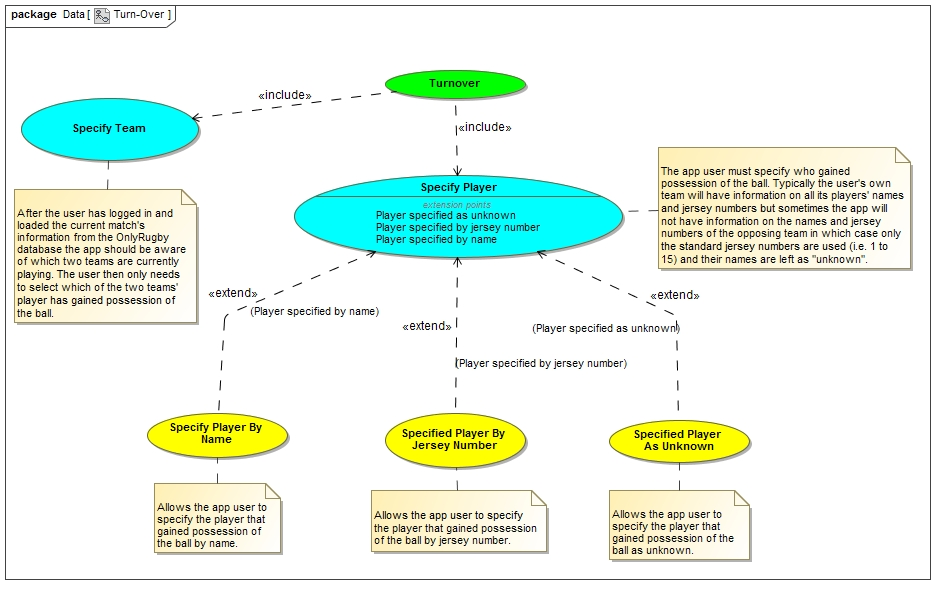
\includegraphics[width=1\textwidth]{./Diagrams/Turn-Over.jpg}\\[0.4cm]
		\end{center}
	\item \textbf{Clean breaks}
		\begin{flushleft}
		This use case will be used to log when clean breaks occur, the player that got the clean break will also be recorded.
		\end{flushleft}
		\begin{center}
		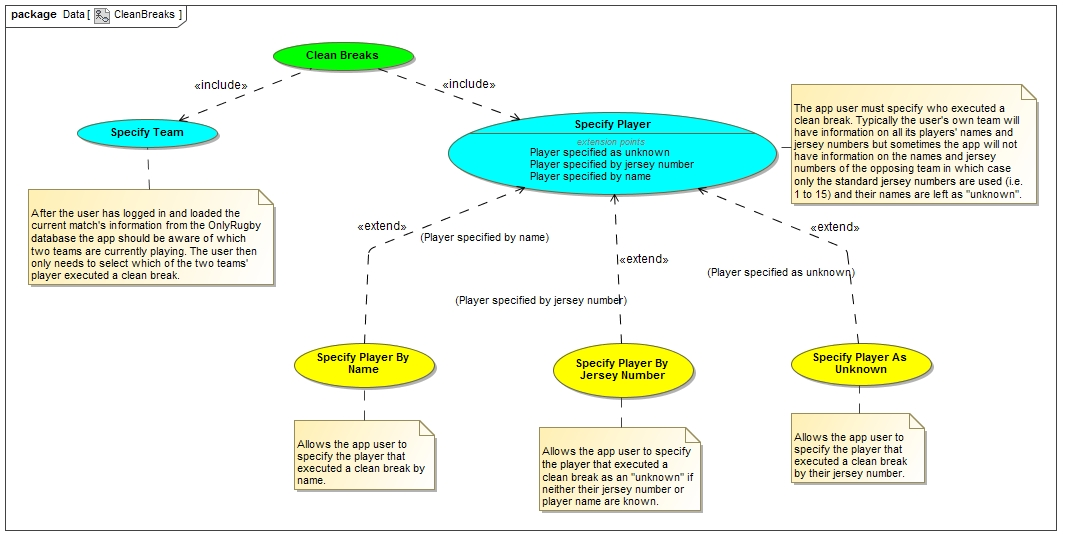
\includegraphics[width=1\textwidth]{./Diagrams/CleanBreaks.jpg}\\[0.4cm]
		\end{center}
	\item \textbf{Offloads}
		\begin{flushleft}
		This use case will be used to log information on when an offload occurs, which team performed the offload, and the identity (name or player number) of the player that performed the offload.
		\end{flushleft}
		\begin{center}
		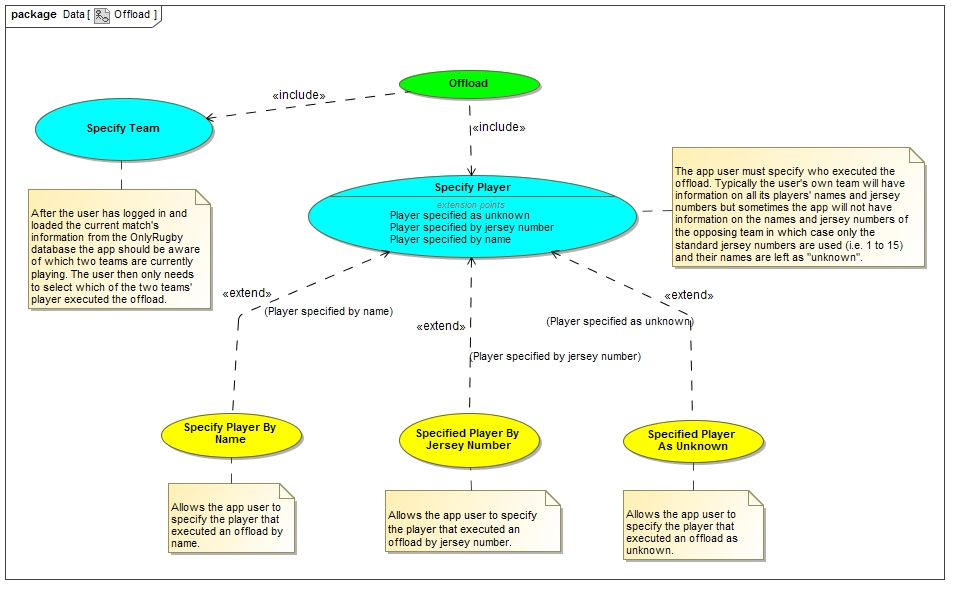
\includegraphics[width=1\textwidth]{./Diagrams/Offload.jpg}\\[0.4cm]
		\end{center}
	\item \textbf{Rucks}
		\begin{flushleft}
		This use case deals with logging any instance of a ruck during match time. When a ruck occurs during a match the OnlyRugby app user can then use this use case to specify which team was defending during the ruck and whether possession of the ball changed during/after the ruck. This use case will also automatically log when a ruck occurs. All this information is then verified by the app user before it is stored in the database. Once stored this information can then be used to give team- and player statistics.
		\end{flushleft}
		\begin{center}
		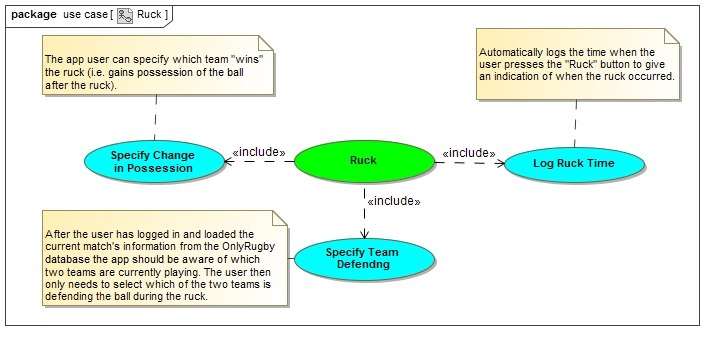
\includegraphics[width=1\textwidth]{./HermanDiagrams/Ruck.jpg}\\[0.4cm]
		\end{center}
\newpage
	\item \textbf{Mauls}
		\begin{flushleft}
			This use case will be used to log how many mauls occurred throughout the match. It will record how many occurred, when they occurred and who won the outcome of the maul (whether there was a turnover ball or not, or if a penalty was conceded).
		\end{flushleft}
		\begin{center}
		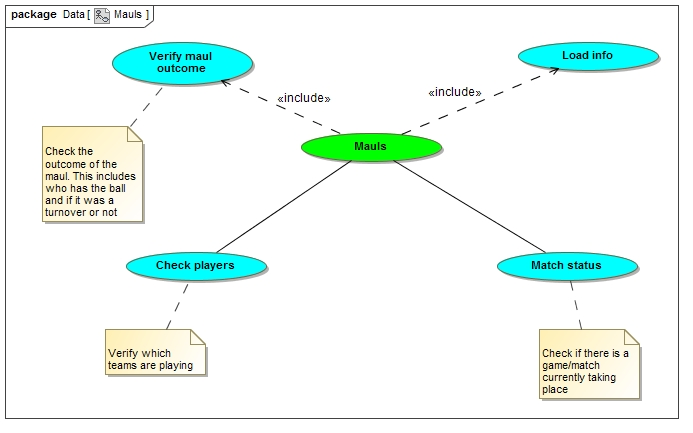
\includegraphics[width=1\textwidth]{./Diagrams/Mauls.jpg}\\[0.4cm]
		\end{center}
\end{itemize}
\newpage
\subsection{Process specification}
The processes followed when using some of the more important functions of the OnlyRugby app system are displayed below:
\begin{itemize}
	\item Log in/ log out
		\begin{center}
  	 	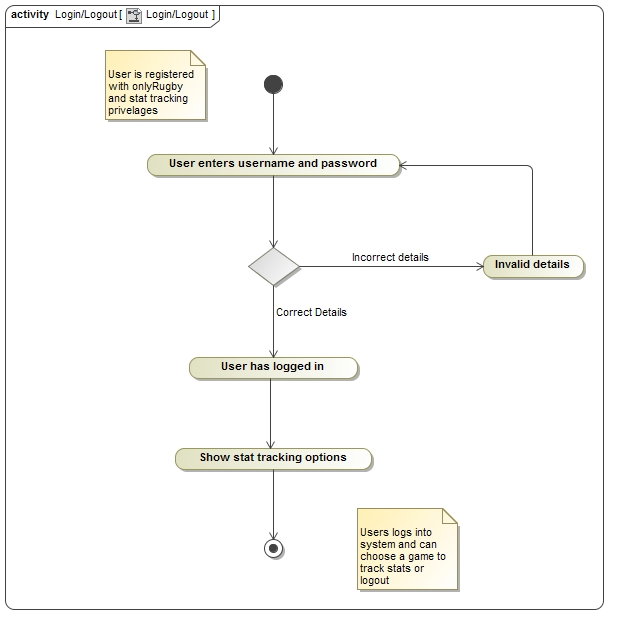
\includegraphics[width=0.6\textwidth] {./Diagrams/Login_LogoutActivityDiagram.jpg}\\[0.4cm]    
		\end{center}
	\item Load info
		\begin{center}
  	 	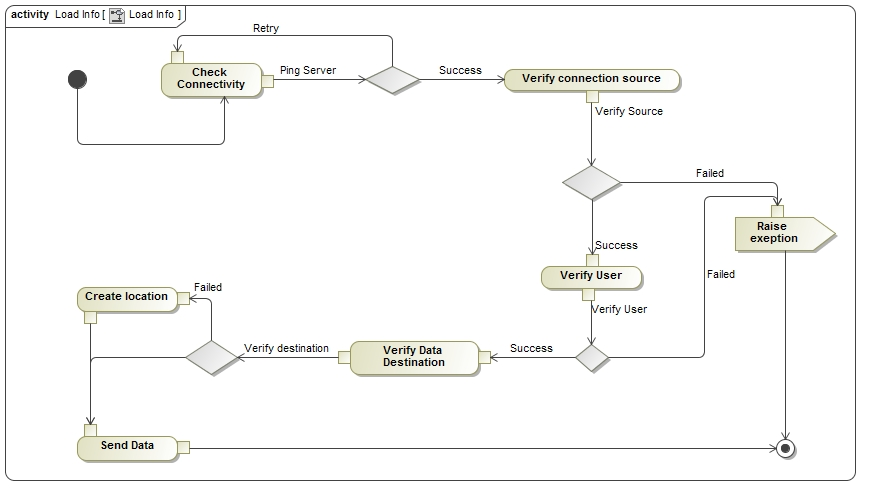
\includegraphics[width=1\textwidth] {./Diagrams/LoadInfoActivityDiagram.jpg}\\[0.4cm]    
		\end{center}
	\item Game time
		\begin{center}
		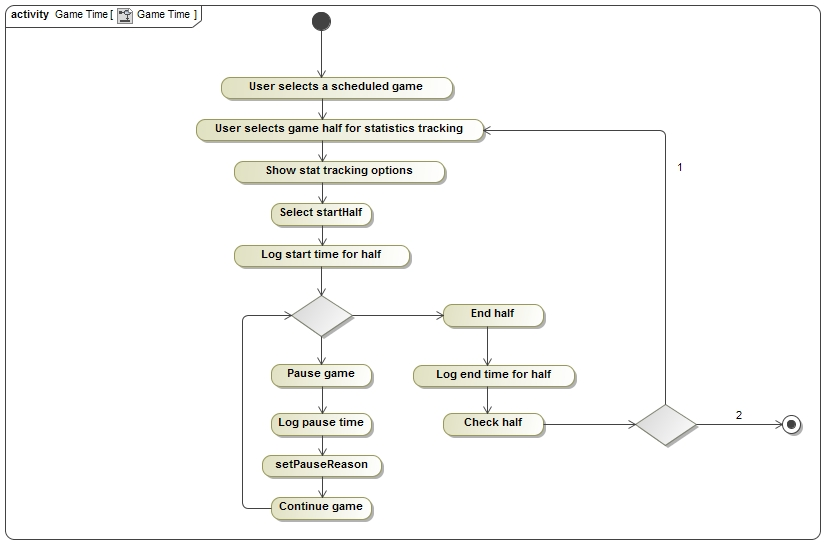
\includegraphics[width=1\textwidth] {./Diagrams/GameTimeActivityDiagram.jpg}\\[0.4cm]
		\end{center}
	\item Scoring
		\begin{center}
		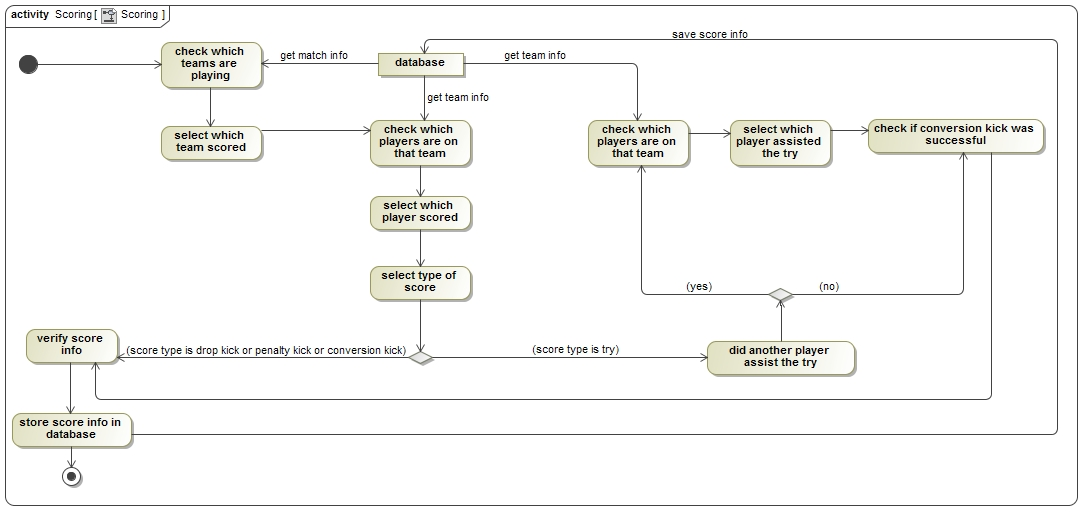
\includegraphics[width=1\textwidth] {./HermanDiagrams/ScoringActivityDiagram.jpg}\\[0.4cm]
		\end{center}
\newpage
	\item Substitutions
		\begin{center}
		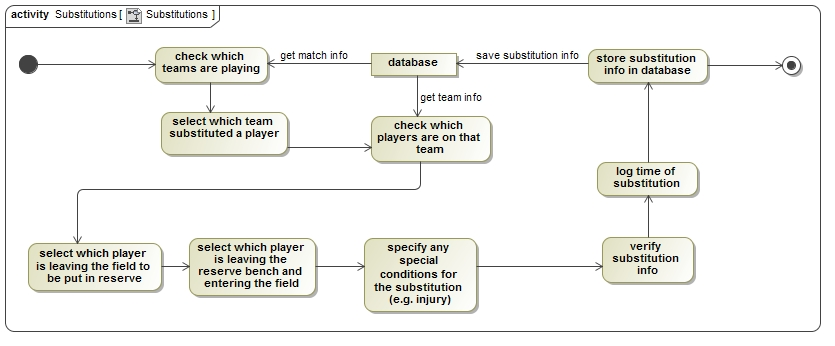
\includegraphics[width=1\textwidth] {./HermanDiagrams/SubstitutionsActivityDiagram.jpg}\\[0.4cm]
		\end{center}
	\item Discipline
		\begin{center}
		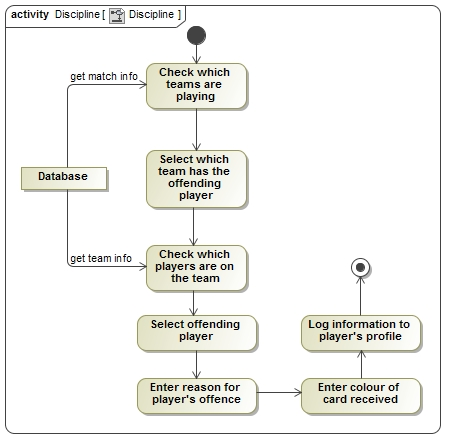
\includegraphics[width=0.6\textwidth] {./Diagrams/DisciplineActivityDiagram.jpg}\\[0.4cm]
		\end{center}
\end{itemize}
\subsection{Domain Model}
	\begin{center}
  	 	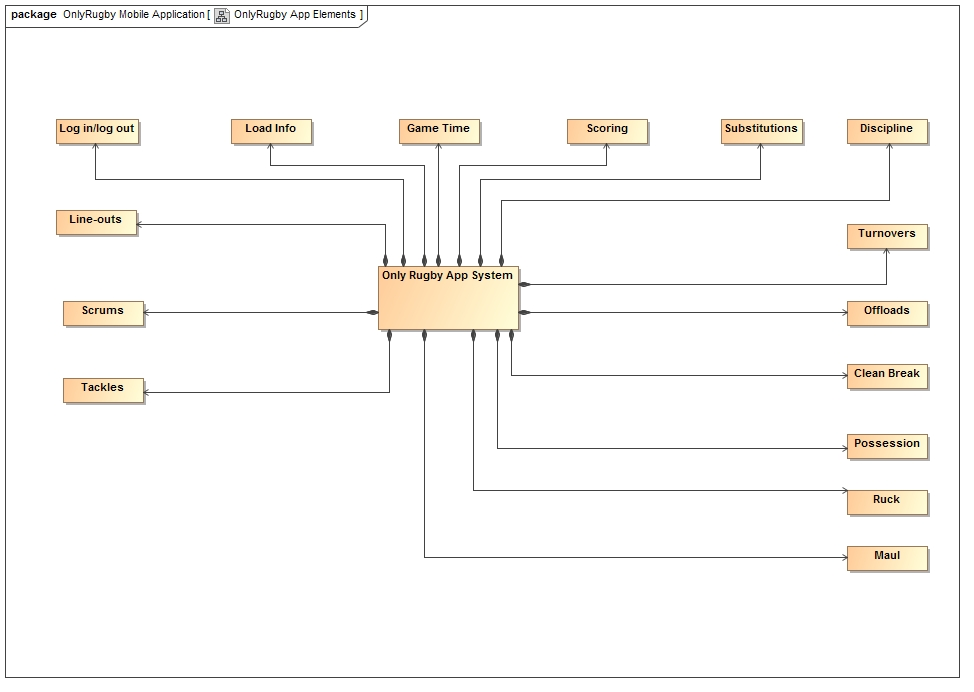
\includegraphics[width=1\textwidth] {./HermanDiagrams/DomainModel.jpg}\\[0.4cm]    
	\end{center}
\index{Vision}
\newpage


\bibliography{myrefs}{} 
\bibliographystyle{ieeetr}
\end{document}
